\section{Implicit and Forceful Data Type Casting}
\begin{frame}<beamer>
    \frametitle{Outline}
    \tableofcontents[currentsection]
\end{frame}

\begin{frame}[fragile]{Implicit Data Type Casting}
\begin{itemize}
	\item {See whether you can work out the answer}
\end{itemize}
\begin{columns}
\begin{column}{0.6\linewidth}
	\begin{lstlisting}[numbers=none, language=c, frame=none]
	char c = 'x';
	double a = c + 5 + 1.3 + 1.73e4;
	\end{lstlisting}
\end{column}
\begin{column}{0.4\linewidth}
\begin{figure}
	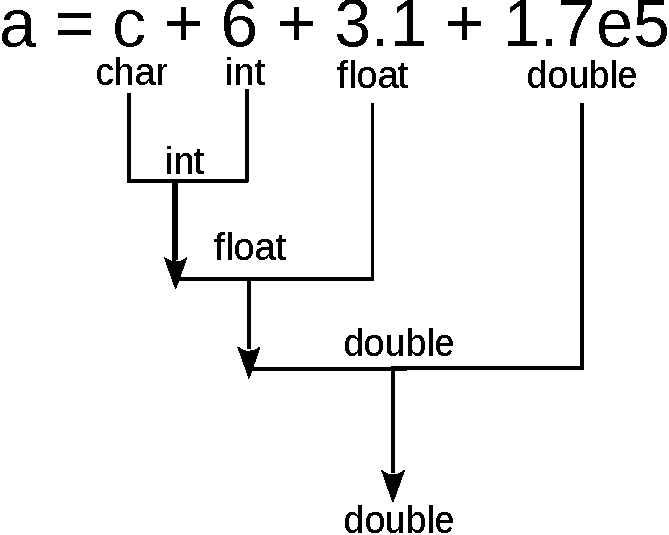
\includegraphics[width=0.9\linewidth]{figs/cast.pdf}
\end{figure}
\end{column}
\end{columns}
\begin{itemize}
	\item {Above type castings are done automatically (implicitly)}
	\item {Code below is risky, rear part will be truncated}
\end{itemize}
	\begin{lstlisting}[numbers=none, language=c, frame=none]
	int a = 0;
	a = 5.1;
	\end{lstlisting}
\end{frame}

\begin{frame}[fragile]{Explicit (forceful) Data Type Casting}
\begin{itemize}
	\item {See whether you can work out the answer}
\end{itemize}
\begin{columns}
\begin{column}{0.6\linewidth}
	\begin{lstlisting}[numbers=none, language=c, frame=none]
	char c = 'x';
	double a = (float)c + (float)5 + 1.3 + 1.73e4;
	\end{lstlisting}
\end{column}
\begin{column}{0.4\linewidth}
\begin{figure}
	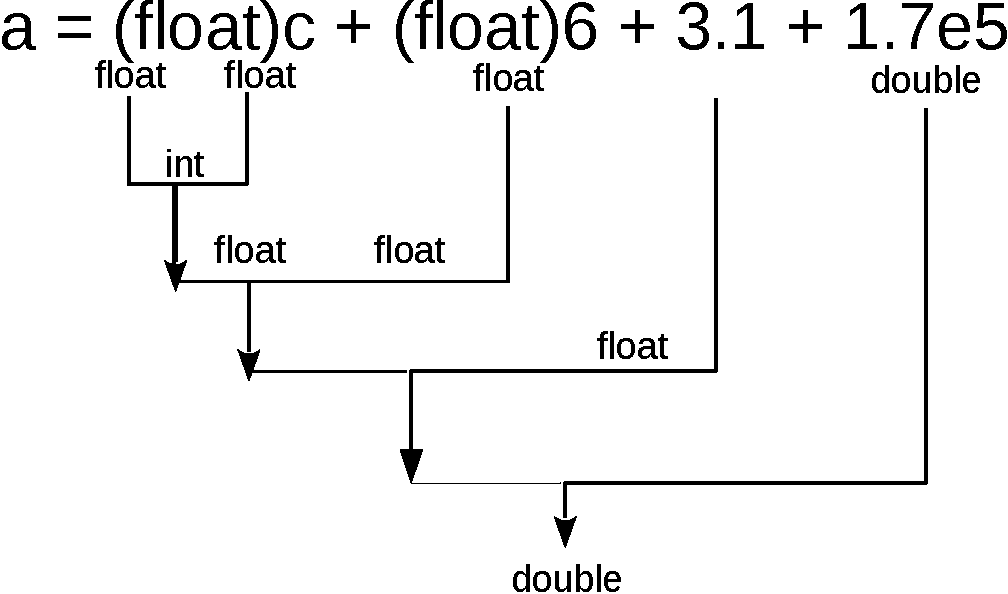
\includegraphics[width=0.9\linewidth]{figs/cast2.pdf}
\end{figure}
\end{column}
\end{columns}
\begin{itemize}
	\item {Above type castings are done forcefully}
	\item {Again it is risky sometimes}
\end{itemize}
\begin{columns}
\begin{column}{0.5\linewidth}
	\begin{lstlisting}[numbers=none, language=c, frame=none]
	int a = 0;
	float b = 5.4;
	a = (int)b;
	\end{lstlisting}
\end{column}
\begin{column}{0.5\linewidth}
	\begin{lstlisting}[numbers=none, language=c, frame=none]
	int a = 0;
	float b = 5.4;
	a = (int)round(b);
	\end{lstlisting}
\end{column}
\end{columns}
\end{frame}